%%%%%%%%%%%%%%%%%%%%%%%%%%%%%%%%%%%%%%%%%%%%%%%%
% 1: Introducción
%%%%%%%%%%%%%%%%%%%%%%%%%%%%%%%%%%%%%%%%%%%%%%%%
\pagenumbering{arabic} % para empezar la numeración con números
\chapter{Introducción}\label{introduccion}


%Desde el comienzo de su historia, la informática ha intervenido en cada aspecto científico y social existente. La dependencia de la sociedad en una ciencia tan reciente resalta la importancia de que sea algo comprensible y comprendido para la sociedad misma.

Como dice M. Lemaire\cite{lemaire2014incorporating}, en una sociedad que está incrementando su dependencia a las nuevas tecnologías\footnote{Aquí, con nuevas tecnologías me refiero a productos y proyectos derivados de la Informática y las \acrfull{TIC} como puede ser los proyectos que detallamos en la sección \ref{estado-arte}.}, es imprescindible que las nuevas generaciones desarrollen la habilidad de pensar de manera crítica sobre tecnología.

El \emph{pensamiento computacional}, como se refiere A. Bundy en \cite{bundy2007computational}, afecta a  investigaciones de casi todas las disciplinas, tanto de ciencias como de humanidades. [...] La informática no solo ha permitido que los investigadores puedan hacer nuevas preguntas, sino también ha permitido aceptar nuevos tipos de respuesta. Por ejemplo, preguntas que requieren el procesamiento de una gran cantidad de datos.

Es necesario comprender la informática y desarrollar el \emph{pensamiento computacional}. Se necesitan desarrollar nuevas tecnologías, nuevo \gls{hardware} y \gls{software} que automatice tareas largas, complejas y con una alta cantidad de cómputo. Tareas que no siempre los humanos podemos resolver de manera directa. Para conseguir esto, muchas veces es necesario programar.

Pero aprender a programar es mencionado como uno de los 7 grandes retos de la educación informática \cite{mcgettrick2005grand} y diversos estudios \cite{renumol2009classification} muestran que las principales dificultades para un alumno cuando está en el proceso de aprender a programar son (a) como empezar un programa; (b) comprensión de la sintaxis específica del lenguaje de programación; (c) comprensión de la lógica\footnote{En este caso me refiero a lógica booleana, o también llamada Álgebra de Boole.} y (d) problemas a la hora de depurar el código escrito.

Aunque a primera vista aprender a programar pueda parecer una tarea ardua y compleja, tiene sus ventajas. En el estudio realizado por J. Siegmund y otros en \cite{siegmund2014understanding}, podemos ver como los participantes mientras comprendían, analizaban y buscaban errores en pequeños trozos de código, daban claras muestras de estar desarrollando actividad cerebral en regiones del cerebro relacionadas con el procesado del lenguaje, la atención y la memoria de trabajo.

De la misma manera, estudios realizados en niños \cite{clements1986effects} de entre 6 y 8 años, muestran que estos demostraron mayor capacidad de atención, más autonomía y un mayor placer por el descubrimiento de nuevos conceptos. En la misma linea, un estudio en niños de infantil \cite{logo-geometry} que utilizaban el \Gls{logo} demostró que los mismos obtuvieron mejores resultados en pruebas de razonamiento, matemáticas o resolución de problemas. Otro estudio más reciernte \cite{liao1991effects} demuestra que aprender a programar (independientemente del lenguaje) a una corta edad, potencia la creatividad y la habilidad de aprendizaje.



\section{Situación actual}
\label{sec:situacion-actual}


Actualmente existen muchos proyectos con el fin de introducir la programación como asignatura obligatoria en Educación Primaria y Secundaria\footnote{{\color{red}En este documento se hablará a menudo de alumnos de Educación Primaria, Secundaria o Bachillerato pero no siempre referido al sistema educativo español. Cada pais tiene un sistema educativo diferente que varía la edad de escolarización de los alumnos. Por generalizar, se tomará la edad y cursos escolares como referencia cuando se hable de Educación Primaria, Secundaria o Bachillerato. En el Apéndice \ref{anexo:edad-educacion} se profundiza más en la diferencia de edad en los principales Sistemas Educativos que pueden ser referenciados, directa o indirectamente, en el presente documento}.}. Estos proyectos vienen respaldados por importantes cambios en los planes de estudios de todo el mundo para enseñar programación\cite{cs-education,madrid-programacion,codigo21, guide-england-computing,chicago-cs}, marcando una clara tendencia social de incluir la programación en los currículos académicos.


Uno de los proyectos más importantes y con más repercusión a nivel global es Code.org\cite{code-org}. Propone una serie de herramientas y juegos diseñados especialmente para que los niños aprendan programación mientras juegan con sus personajes favoritos de películas y videojuegos. Todo ello acompañado de una infraestructura para que profesores puedan incluir estos proyectos en las aulas, y padres en sus casas.
Su proyecto \emph{Hora del código}\cite{hour-of-code} consigue reunir a niños de todas las edades una hora al día para que la inviertan en programar.
Code.org cuenta con decenas de millones de estudiantes de más de 180 países, disponible en más de 30 idiomas. De manera gratuita, cualquiera puede aprender a programar en eventos que se realizan por todo el mundo (figura \ref{fig:map-hour-code}). Code.org está apoyado por grandes compañías y persanalidades a nivel global como puede ser Microsoft, Google, el Presidente Barack Obama, Mark Zuckerberg, Bill Gates o Walt Disney Company. En la sección \ref{sec:Code.org} se abordará más detalladamente las diferentes formas que tiene Code.org de enseñar a programar.


\begin{figure}[!ht]
	\begin{centering}
		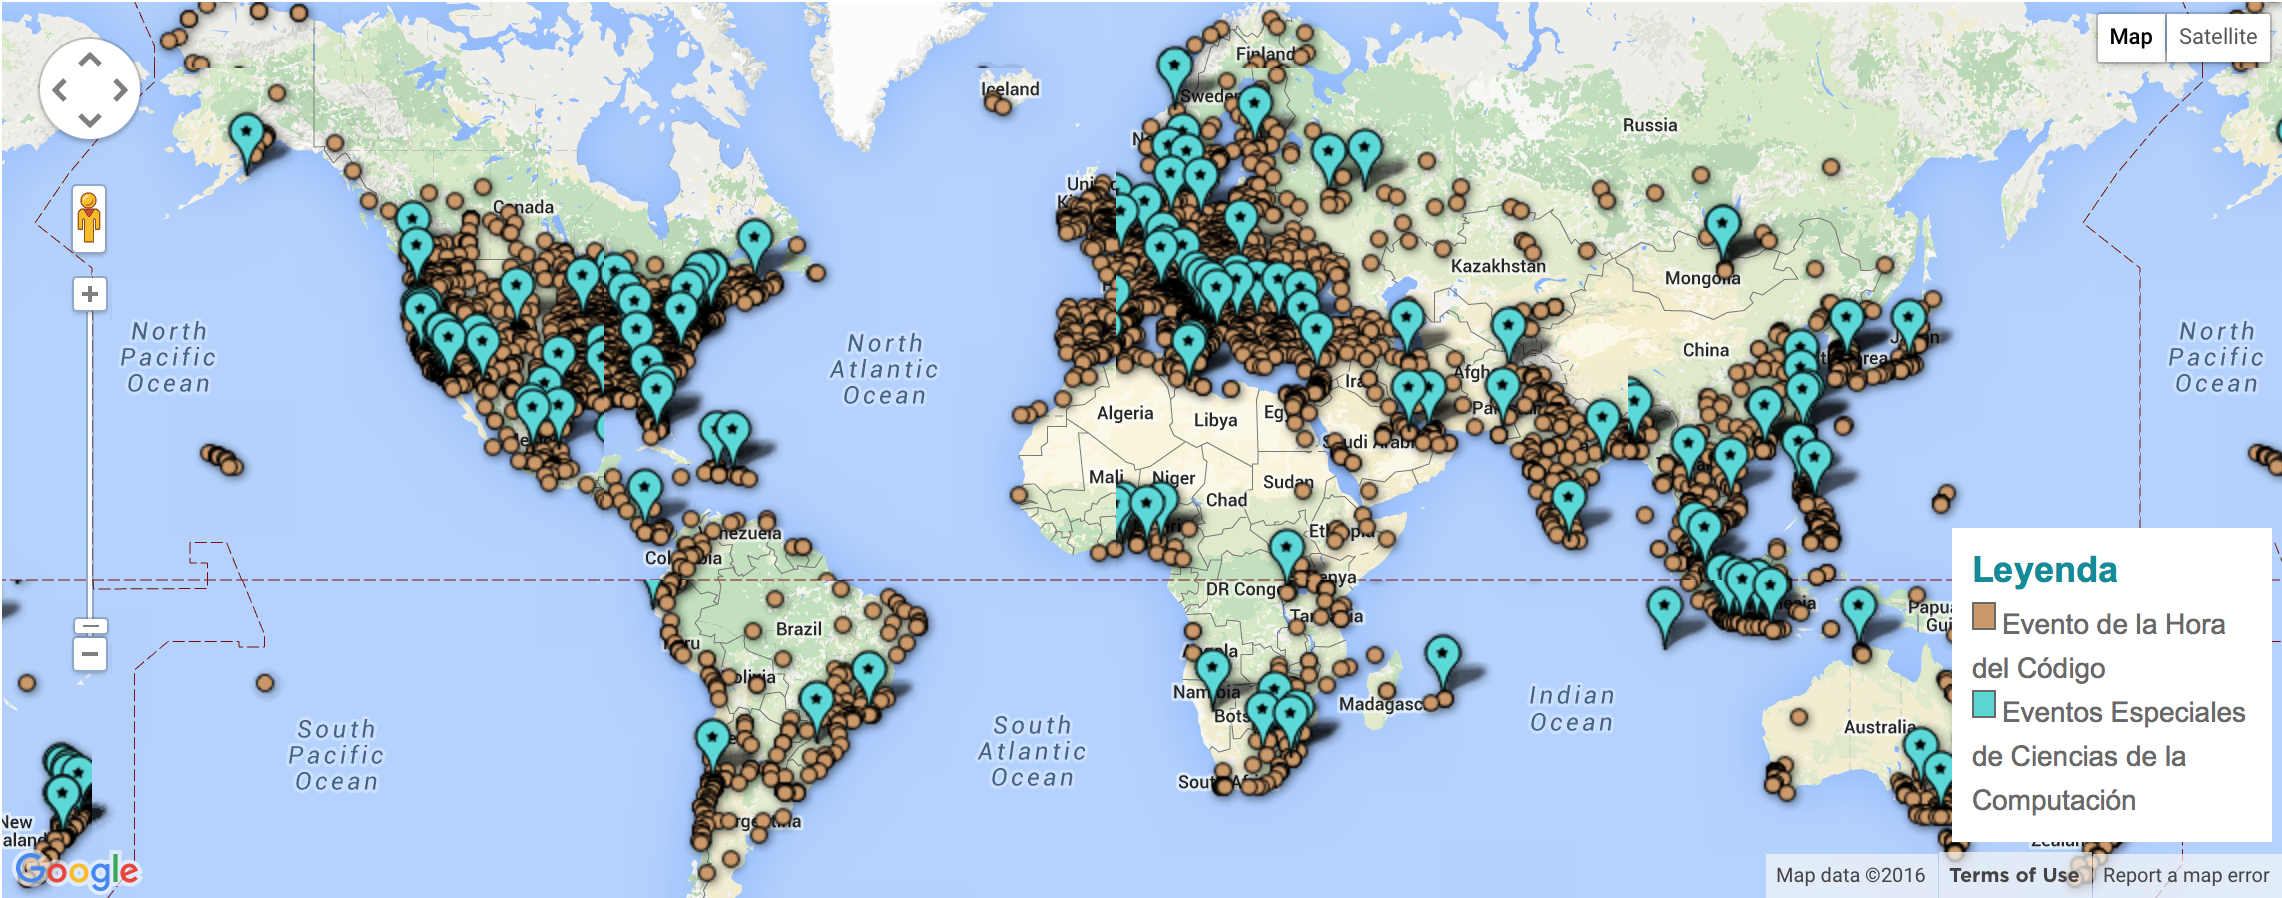
\includegraphics[width=0.8\textwidth]{images/map-hour-code.png}
			\caption{Mapa de visualización de eventos de llevados a cabo por el proyecto \emph{Hora del código} alrededor del mundo. Actualmente 198,473 en todo el mundo, 1,839 en España. Obtenido de \cite{hour-of-code}.}
				\label{fig:map-hour-code}
	\end{centering}
\end{figure}


A nivel europeo, la \Gls{com-euro}\cite{ec-code-week} ha promovido durante el año 2015 la \emph{EU Code Week}\cite{code-week} como parte de su Estrategia para la Educación y la Formación 2020. Este proyecto consistió en eventos de una semana de duración en la que se enseñaba informática y programación en lugares de toda Europa\footnote{En España, se realizaron eventos dentro del marco del proyecto \emph{EU Code Week} en Madrid, Sevilla, Murcia, Asturias, Canarias, Cantabria, Zamora, Cataluña, Ceuta, Badajoz, La Rioja, País Vasco y Valencia.}.


\section{Usando la electrónica y la robótica para enseñar a programar}
\label{sec:electronica-robotica}


Una forma bastante extendida para enseñar a programar en las aulas es con robótica y electrónica. Muchos proyectos de robótica animan al alumno a formarse en dos grandes materias: electrónica y programación. Cuando un estudiante tiene que hacer que un robot se mueva, tendrá que aprender a programar su comportamiento, pero también deberá conocer y en algunos casos incluso crear nuevas piezas para su correcto funcionamiento y personalización.

Existen proyectos como Arduino\footnote{Arduino es una placa base con un microprocesador que es capaz de analizar entradas de información (un sensor, un botón o incluso una notificación de Twitter (\url{www.twitter.com}) y convertirlo en una respuesta como el activar un robot o encender un led. Todo esto acompañado de un software facil de programar. El proyecto es completamente \emph{\gls{open-source}}.}\cite{arduino} y Raspberry Pi\footnote{Raspberry Pi es un ordenador del tamaño de una tarjeta de crédito. También se provee un Sistema Operativo \emph{Open Source} (aunque este puede ser cambiado). Su funcionamiento es sencillo de programar en Scratch\cite{scratch} o Python\cite{python,lutz2013learning}.}\cite{raspberry-pi} que proporciona {\color{red}los elementos y materiales} básicos para poder crear nuevos proyectos.

En concreto, una de las meta originales de Raspberry Pi es conseguir que los niños aprendan a programar y conozcan como funciona realmente un ordenador. Tanto Arduino como Raspberry Pi pueden adquirirse a un bajo precio, lo cual facilita la adquisición de los mismos por parte de instituciones de enseñanza o particulares. Esto ha facilitado la alta inclusión de estos dos proyectos en las aulas.

Otro proyecto que también está muy extendido en las aulas es Lego Mindstorm EV3 y NXT\cite{lego-mindstorm}. Dos kits de iniciación a la robótica con Lego. Permite al estudiante crear con piezas de lego un robot y programar su comportamiento. Los robots suelen tomar forma de brazo robótico o de vehículo capaz de seguir lineas pintadas en el suelo haciendo uso de sensores. Toda este material robótico viene acompañado de un software para programar el comportamiento de los diferentes componentes del robot y un estilo de programación con bloques\cite{lego-mindstorm-programar}, al estilo Scratch.


{\color{red}
Esto es suficiente?
No se si debería ponerme a hablar de Moway y robomind y todo eso si ya en el estado del arte se hablará ampliamente de eso...
}



\section{Proyecto Descubre la programación}
\label{sec:descubre}

\Gls{descubre}\cite{descubre} es un proyecto diseñado en la Facultad de Informática de la Universidad de Murcia y tiene como objetivo ayudar a los alumnos de Secundaria y Bachillerato a que desarrollen sus capacidades descubriendo lo que es la informática y aprendiendo a programar. Así como fomentar la inclusión del aprendizaje de la programación en secundaria y bachillerato.

Para ello, en un mismo sitio web, se integra (a) un conjunto de tutoriales de programación (figura \ref{fig:descubre-aprende}); (b) una herramienta que permite programar (figura \ref{fig:descubre-crea}) y realizar ejercicios o retos propuestos (figura \ref{fig:descubre-retos}) y (c) una pequeña red social que permite publicar y compartir con el resto de compañeros los programas realizados (figura \ref{fig:descubre-explora}). Adiccionalmente se puede consultar las estadísticas de aprendizaje (figura \ref{fig:descubre-perfil}) y tiempo dedicado (figura \ref{fig:descubre-estadisticas}) en la plataforma, tanto por el alumno como por el profesor. De esta manera se permite que los profesores puedan utilizar Descubre en las aulas y realizar un seguimiento de la dedicación y progreso del alumno.

En cuanto a la herramienta para desarrollar programas, el lenguaje utilizado es \gls{ijava}\cite{sanchez2009ijava} y ha sido desarrollado por J. A. Sánchez Laguna. iJava es un lenguaje imperativo basado en \Gls{java} y comparte su sintaxis, aunque se han eliminado todos los componentes del lenguaje Orientado a Objetos. También incorpora un conjunto reducido de funciones de librería clasificadas en los tres grupos siguientes: númericas, entrad/salida y gráficas\footnote{Si el lector está interesado en aprender más sobre este lenguaje, puede consultar \cite{sanchez2009ijava} o \cite{descubre-lenguaje}.}.

A modo de ilustración, podemos ver el código \ref{code:hello-world}, un programa que imprime por pantalla la cadena "Hello World". En el código \ref{code:circulos-color-raton} podemos ver un programa un poco más complejo que dibuja círculos de colores en la pantalla según la posición del ratón. En la figura \ref{fig:salida-code-circulos-color-raton} se puede ver la salida de este último programa.


\begin{lstlisting}[language={Java}, label={code:hello-world}, caption={Programa básico en iJava imprimiendo la cadena "Hello World".}]
void main(){
  print("Hello World");
}
\end{lstlisting}


\begin{lstlisting}[language={Java},label={code:circulos-color-raton}, caption={Programa en iJava que dibuja un circulo de un color diferente según la posición en la pantalla en la que se encuentra el ratón.}]
void main() {
  //repetimos en bucle la función 'draw'
  animate(draw);
}

void draw() {
  //coloreamos el circulo según la posición del raton
  fill(mouseX, mouseY, 0); //valores RGB
  //dibujamos una elipse con radio 50
  ellipse(mouseX, mouseY, 50,50);
}
\end{lstlisting}


La sintaxis de iJava se parece a muchos de los lenguajes modernos y más utilizados (al ser un subconjunto de la sintaxis de Java), lo cual simplifica el aprendizaje cuando se intenta aprender un nuevo lenguaje. También, gracias a la librería gráfica y matemática, los programas se simplifican mucho en cuanto a complejidad y longitud. De esta manera se consigue aligerar la carga de trabajo que tiene que realizar el alumno para conseguir hacer un programa vistoso, haciendo que la actividad de programar sea más atractiva.


\begin{figure}[!ht]
	\begin{centering}
		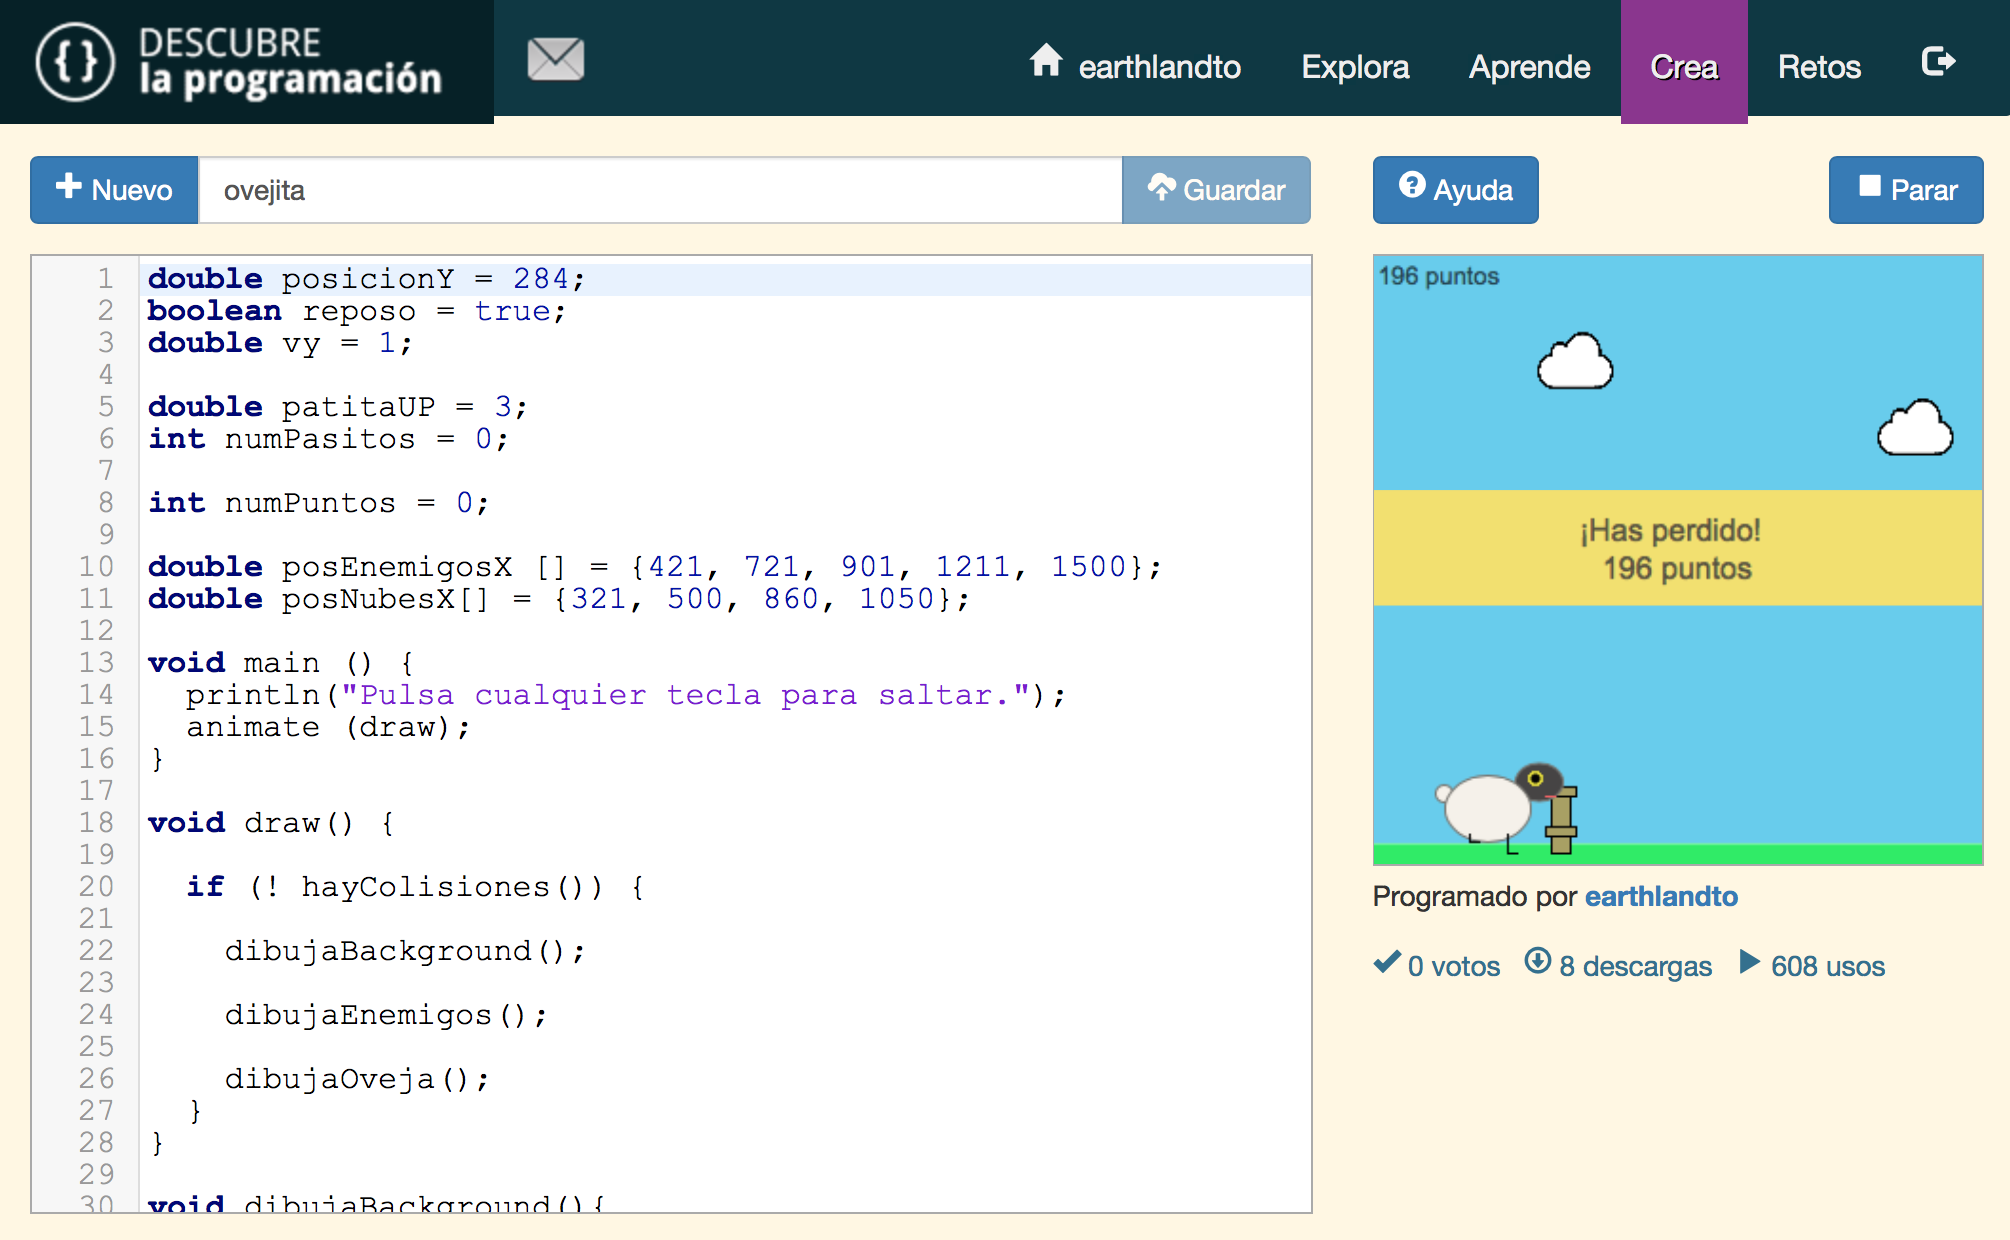
\includegraphics[width=0.7\textwidth]{images/descubre-crea.png}
				\caption{Sección \emph{Crea} del proyecto \Gls{descubre}. Obtenido de \cite{descubre}.}
				\label{fig:descubre-crea}
	\end{centering}
\end{figure}



\begin{figure}[!ht]
	\begin{centering}
		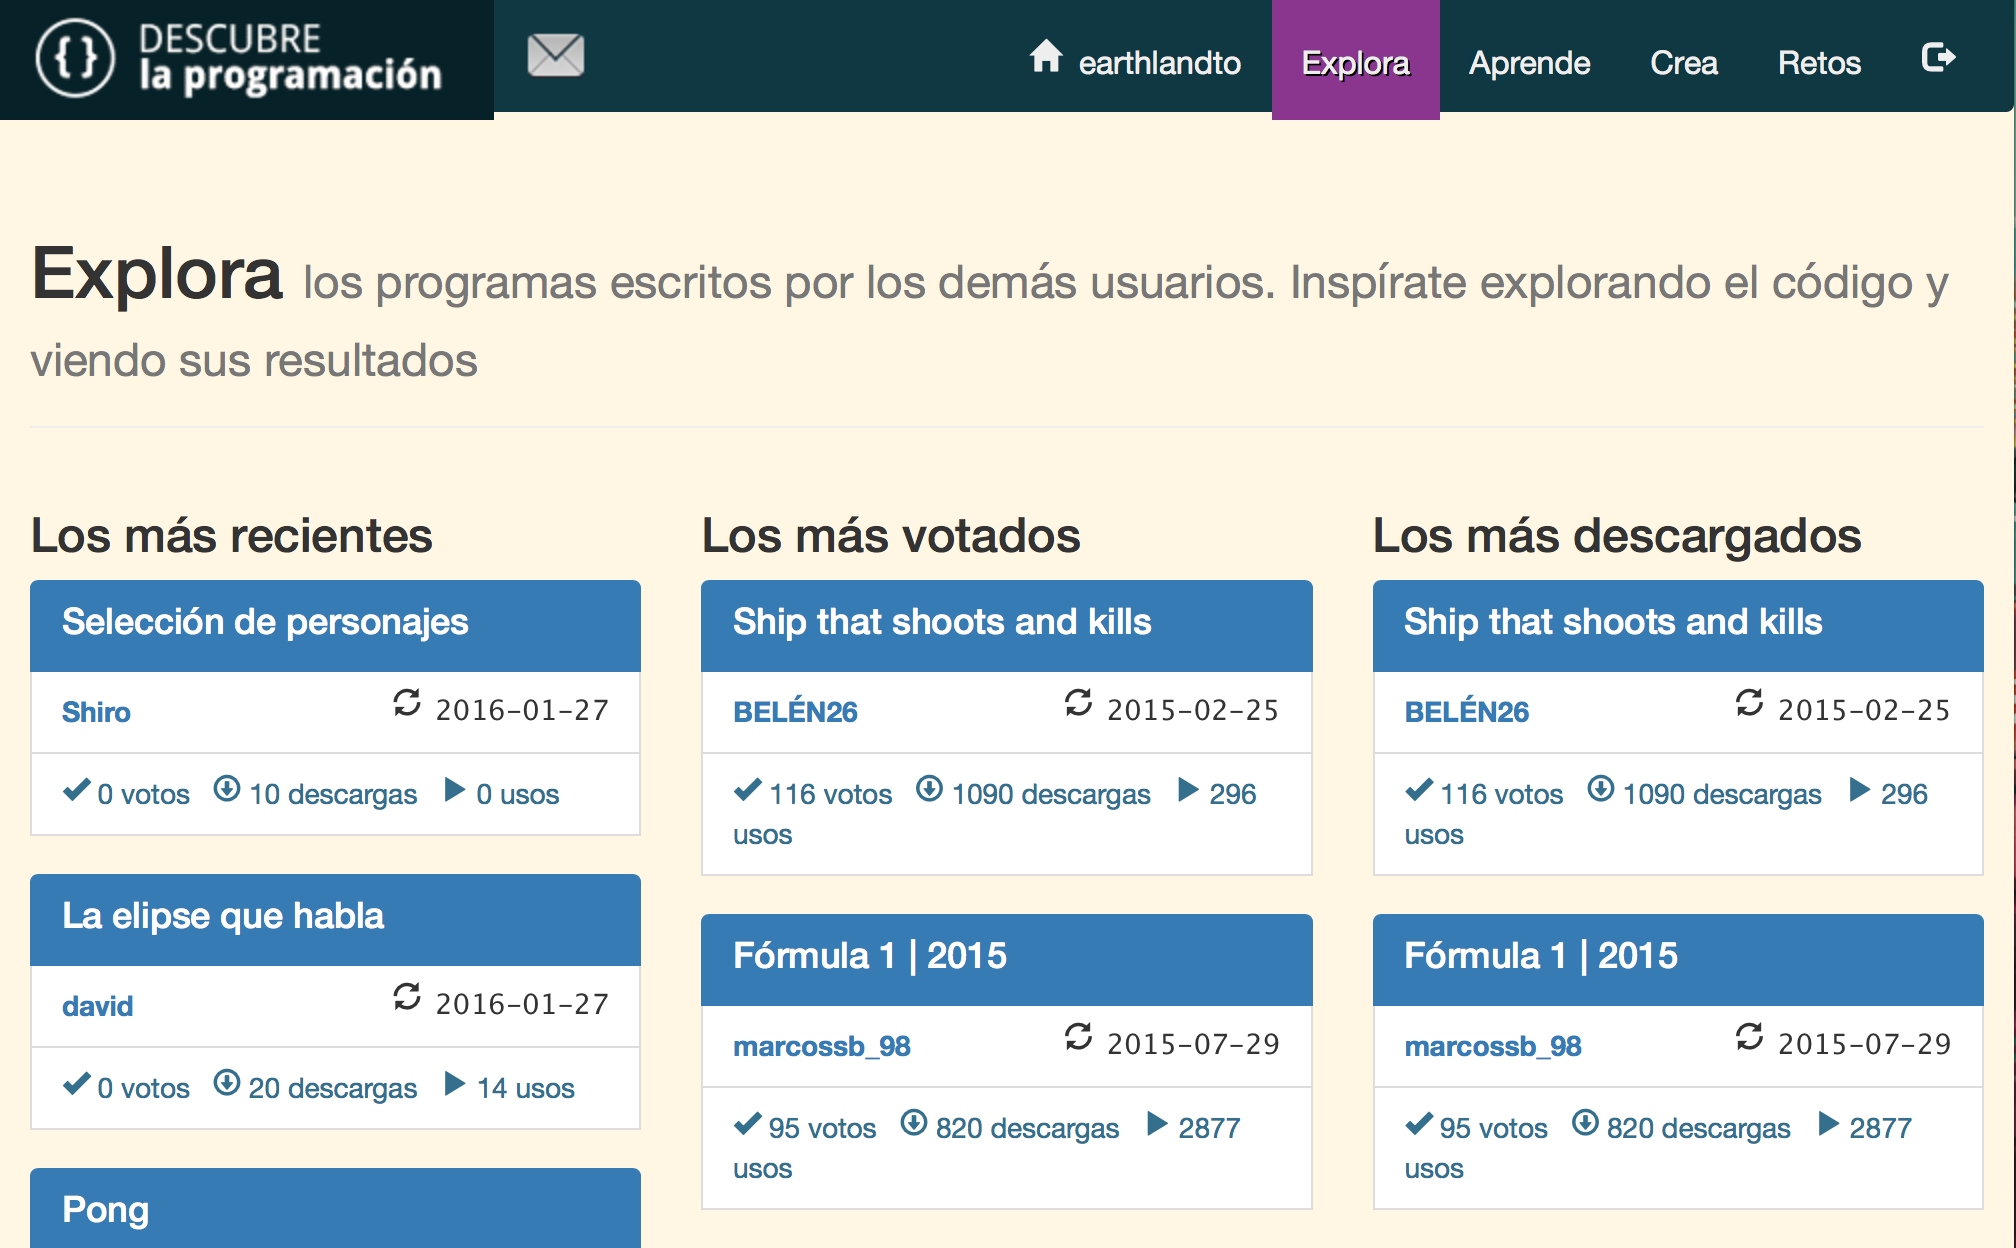
\includegraphics[width=0.5\textwidth]{images/descubre-explora.png}
				\caption{Sección \emph{Explora} del proyecto \Gls{descubre}. Obtenido de \cite{descubre}.}
				\label{fig:descubre-explora}
	\end{centering}
\end{figure}



\begin{figure}[!ht]
	\begin{centering}
		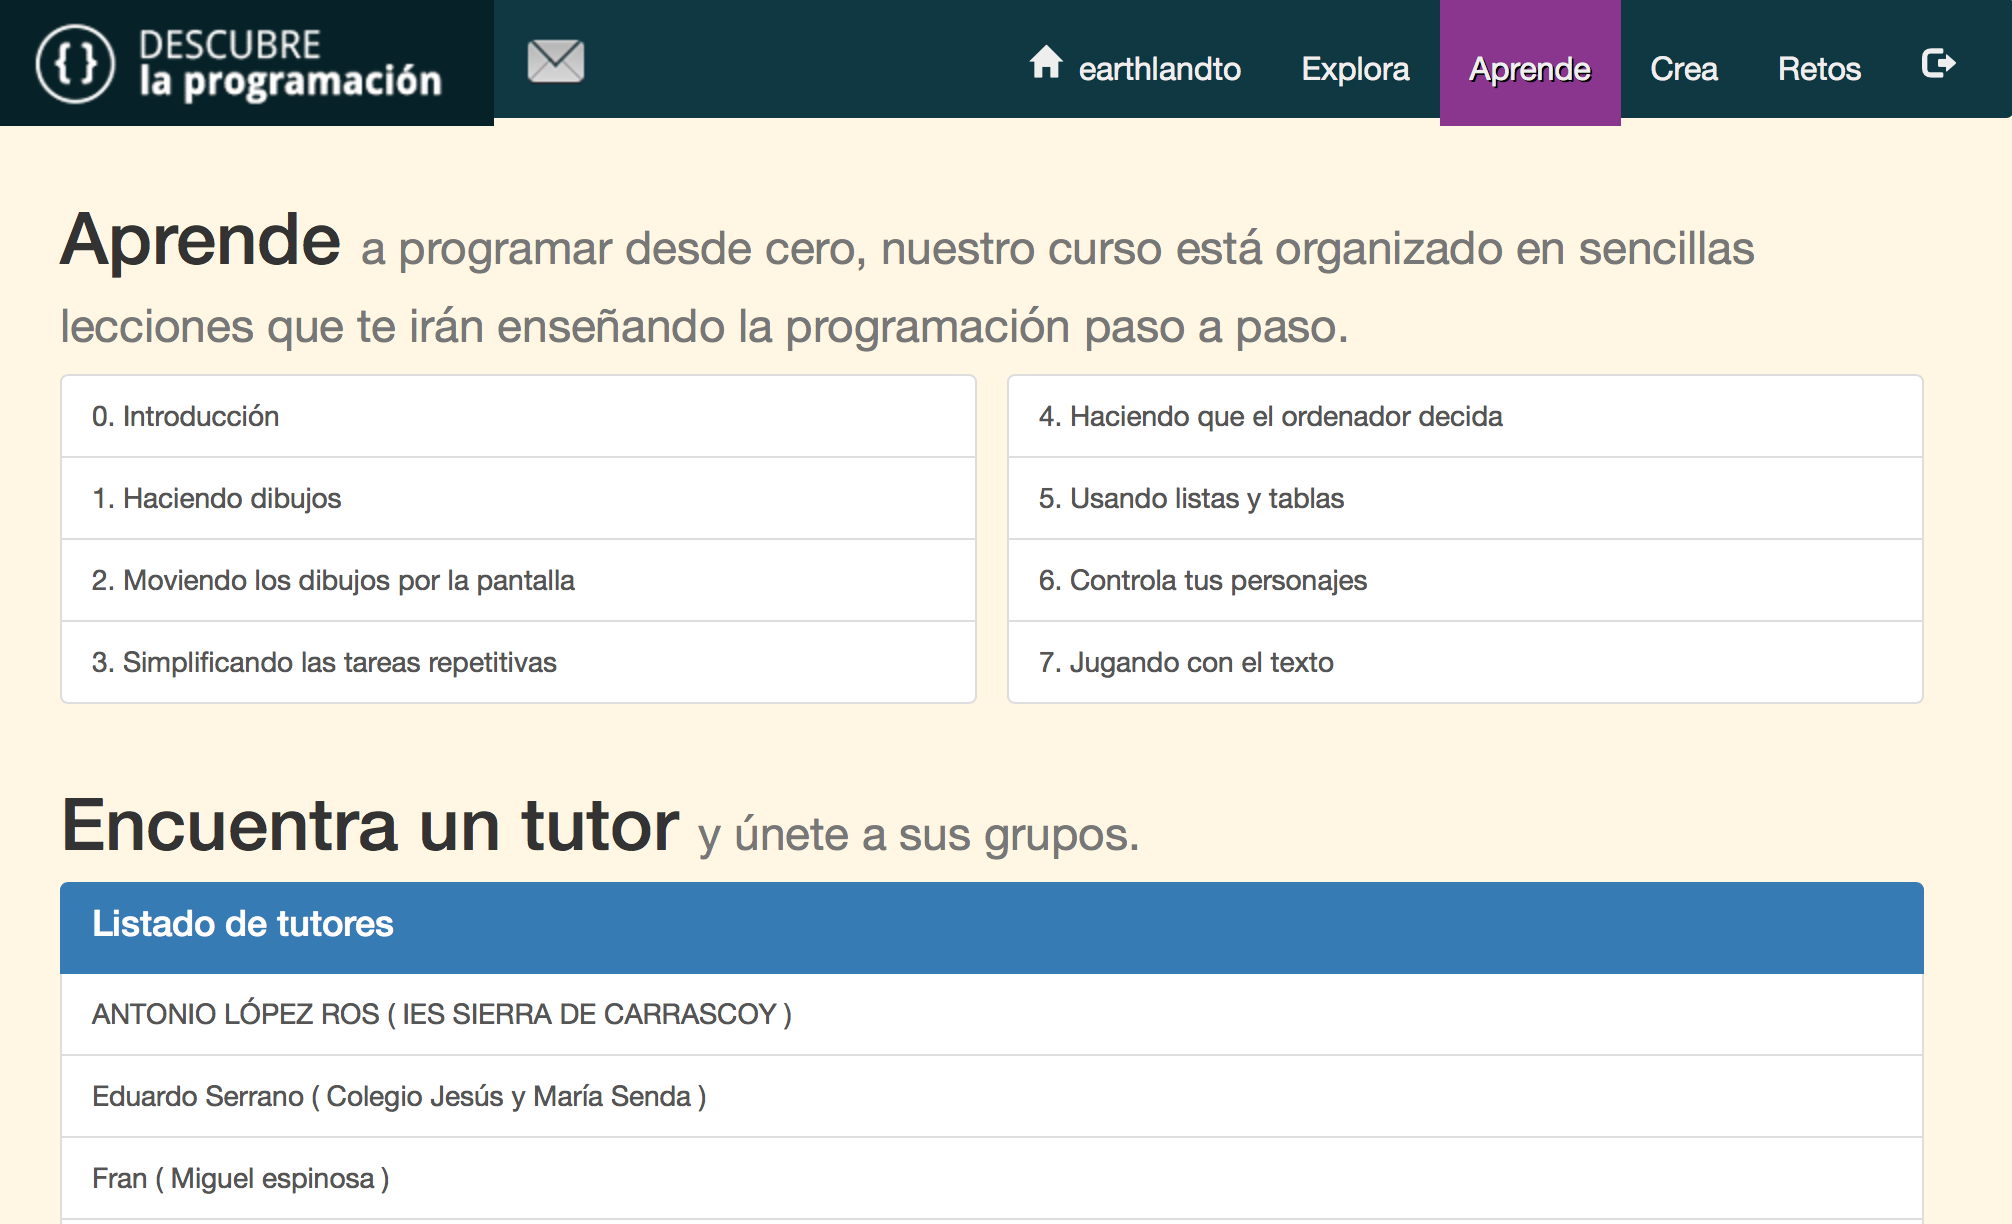
\includegraphics[width=0.5\textwidth]{images/descubre-aprende.png}
				\caption{Sección \emph{Aprende} del proyecto \Gls{descubre}. Obtenido de \cite{descubre}.}
				\label{fig:descubre-aprende}
	\end{centering}
\end{figure}


\begin{figure}[!ht]
	\begin{centering}
		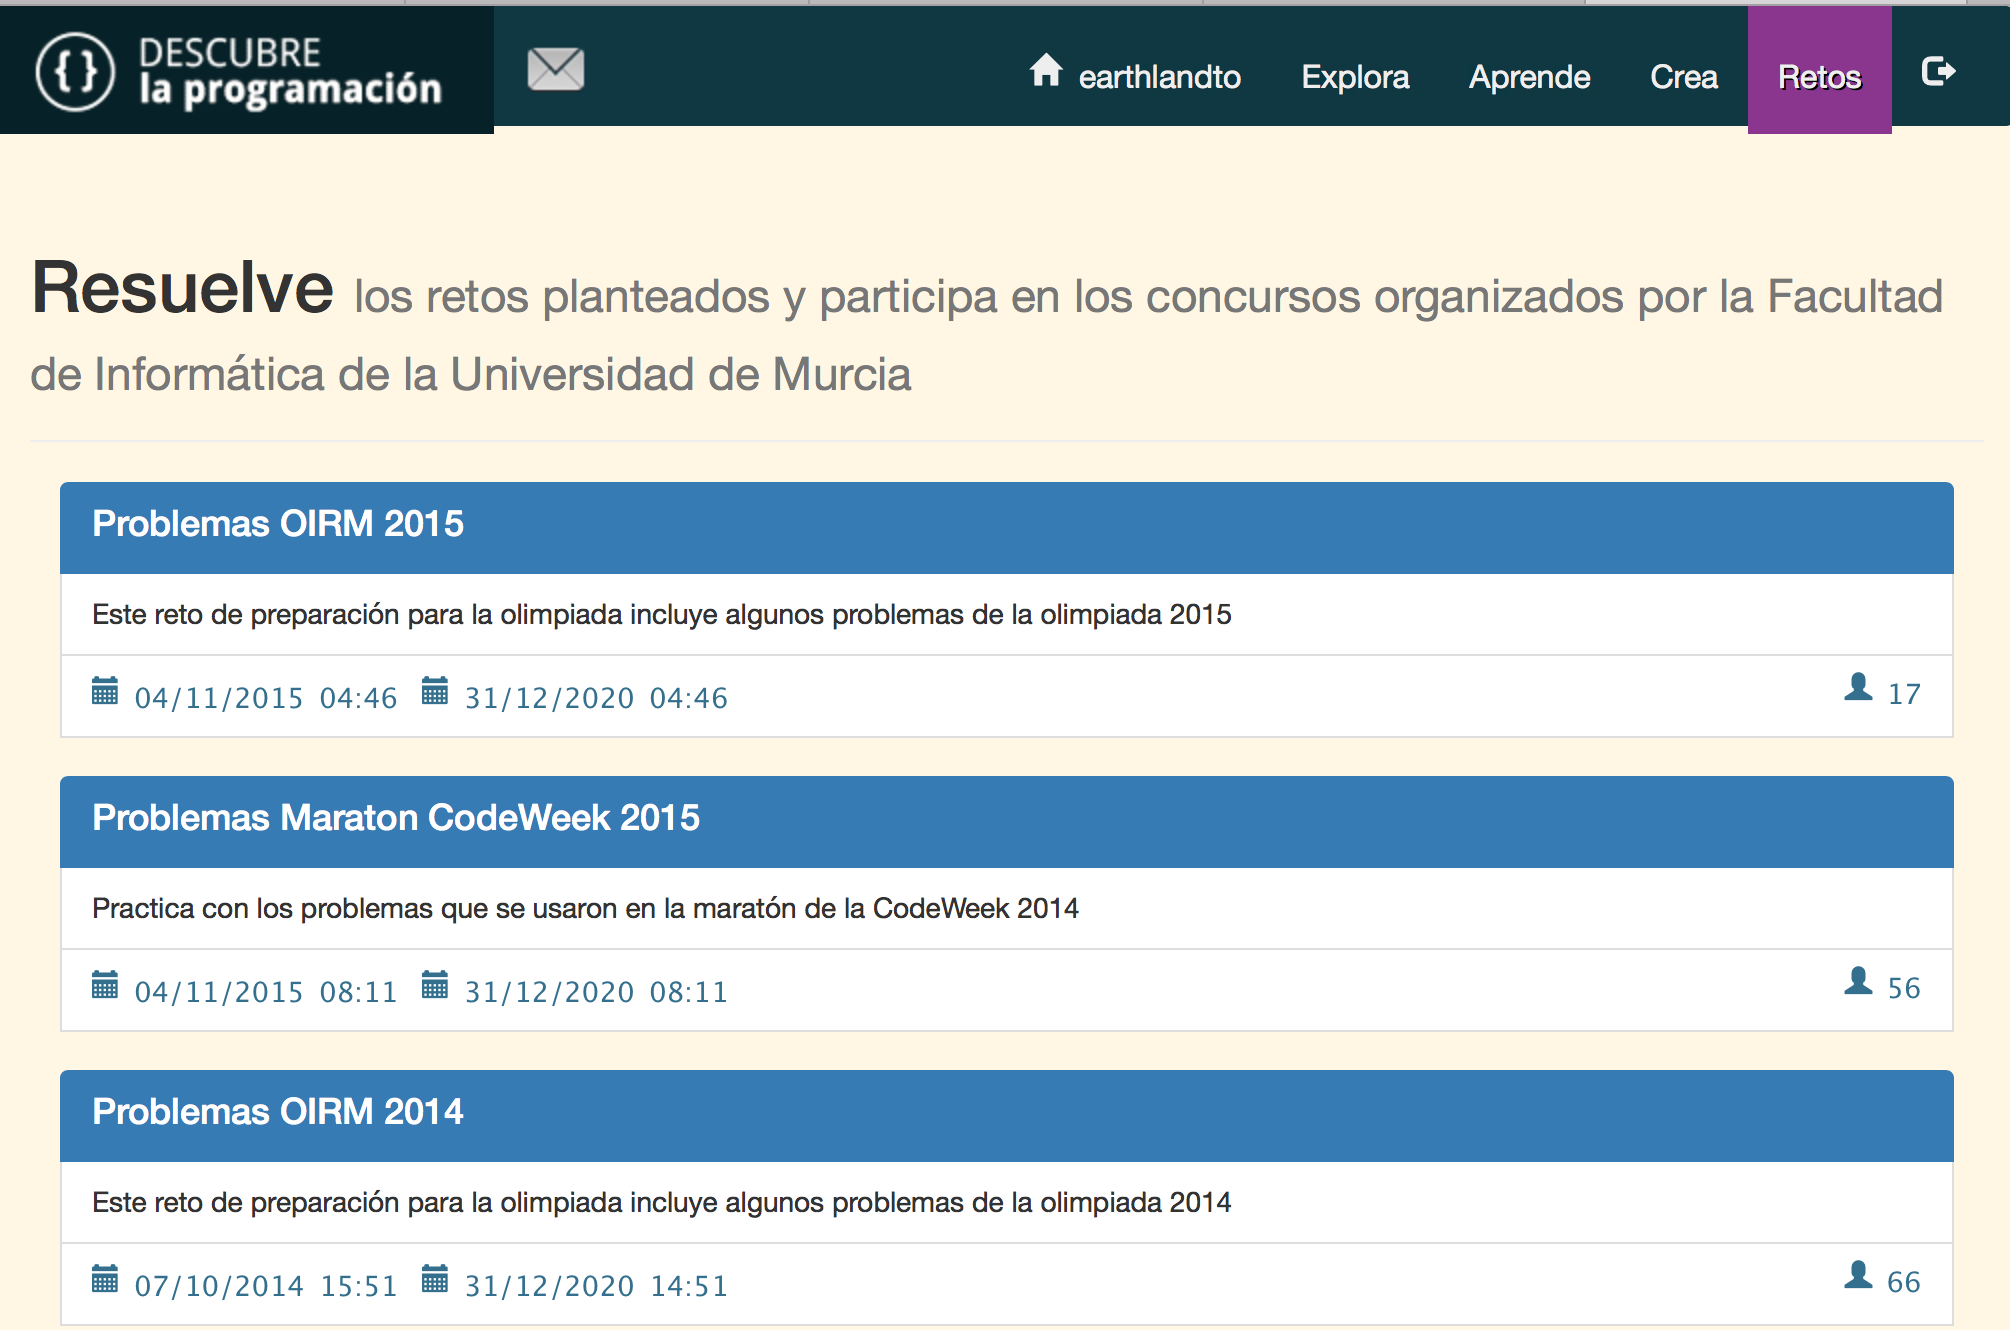
\includegraphics[width=0.5\textwidth]{images/descubre-retos.png}
				\caption{Sección \emph{Retos} del proyecto \Gls{descubre}. Obtenido de \cite{descubre}.}
				\label{fig:descubre-retos}
	\end{centering}
\end{figure}


\begin{figure}[!ht]
	\begin{centering}
		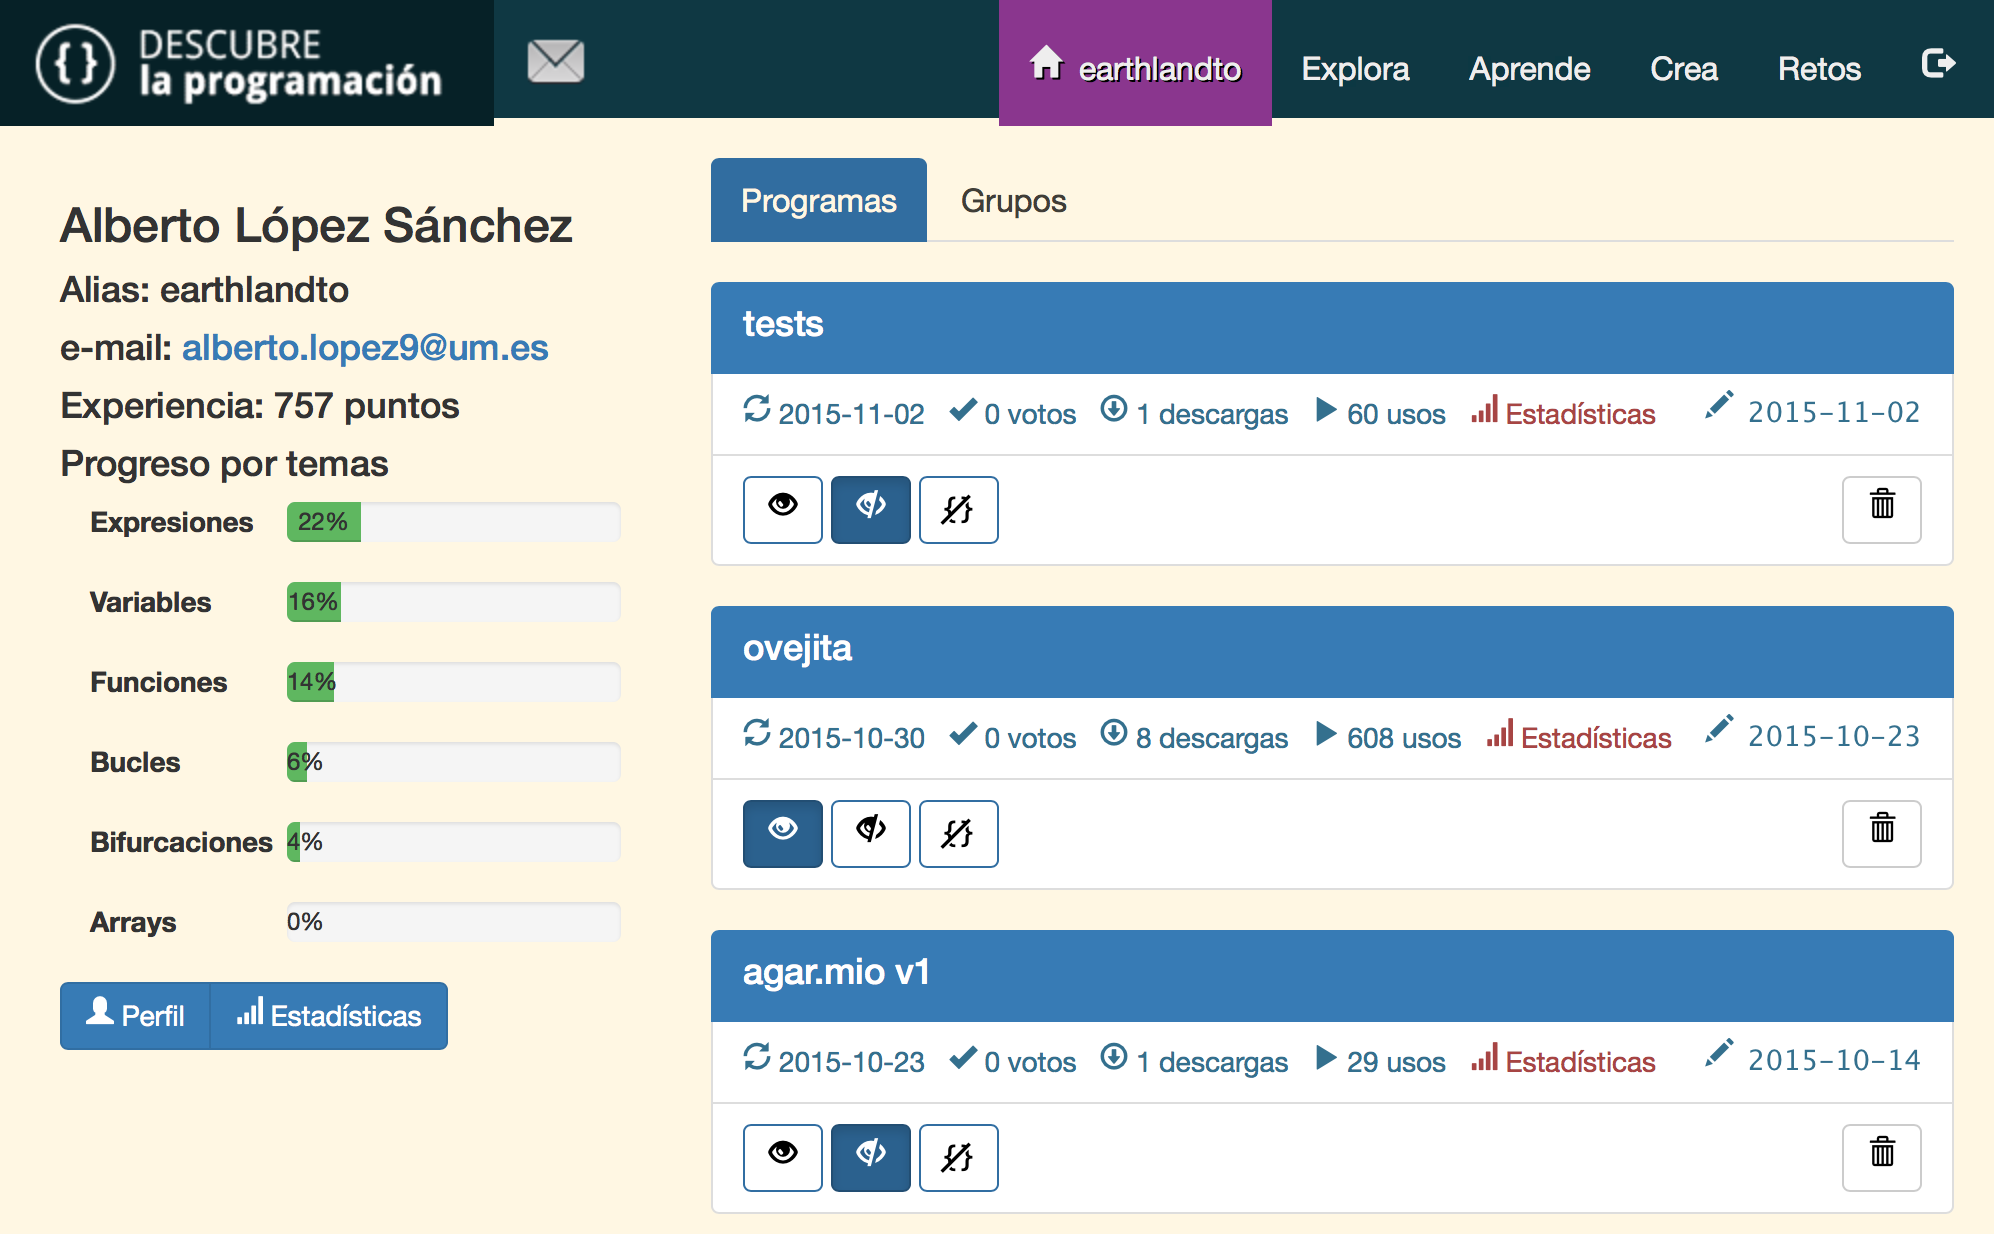
\includegraphics[width=0.5\textwidth]{images/descubre-profile.png}
				\caption{Vista del perfil de usuario del proyecto \Gls{descubre}. Obtenido de \cite{descubre}.}
				\label{fig:descubre-perfil}
	\end{centering}
\end{figure}


\begin{figure}[!ht]
	\begin{centering}
		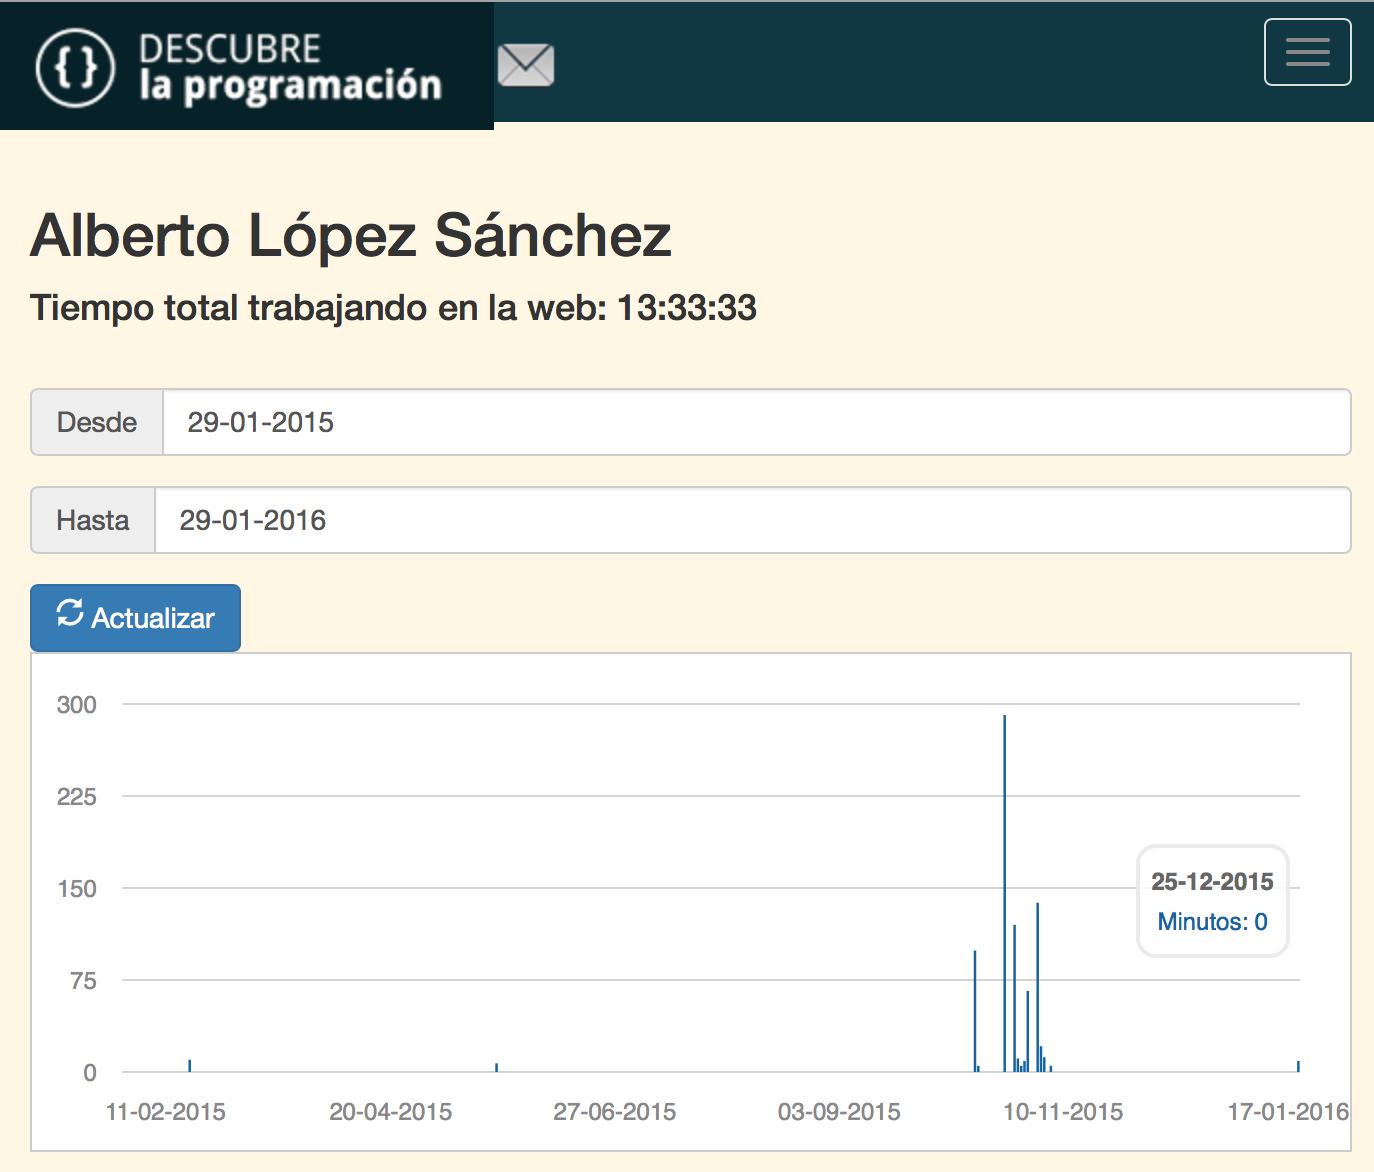
\includegraphics[width=0.5\textwidth]{images/descubre-statistics.png}
				\caption{Sección de estadísticas del usuario del proyecto \Gls{descubre}. Obtenido de \cite{descubre}.}
				\label{fig:descubre-estadisticas}
	\end{centering}
\end{figure}


\begin{figure}[!ht]
	\begin{centering}
		
\includegraphics[width=0.5\textwidth]{images/salida-code-circulos-color-raton.png}
			\caption{Salida del programa escrito en iJava ejecutado por el código \ref{code:circulos-color-raton}.}
				\label{fig:salida-code-circulos-color-raton}
	\end{centering}
\end{figure}





\section{Motivación y enfoque del proyecto}
\label{sec:motivacion}

Las nuevas tecnologías están haciendo que cada vez más gente de todas las edades se interese por la informática, y más concretamente por la programación. Poco a poco la informática deja de ser cosa de un grupo selecto {\color{red}de gente que entiende su funcionamiento}.

Como ya hemos comentado anteriormente, existe un movimiento que pretende introducir la informática y la programación en las aulas. Se han demostrado los beneficios de enseñar a programar en una edad escolar temprana.

Es en este momento cuando se hace imprescindible tomar decisiones acertadas. Aprender a programar en edades pre-universitaria debe ser algo accesible a cualquier estudiante, independiente de su condición o los antecedentes del mismo. Igualmente, los conceptos de programación deben ser presentados de manera, incremental, empezando por los más simples para luego ampliar a conceptos más complejos, como defiende L. Fernandez y otros en \cite{fernandez2002analisis}.

El proyecto se enfocará desarrollando un simulador de robot de dos ruedas en el que los alumnos puedan programar su comportamiento. Se ofrece una librería de funciones para simplificar la interacción con el mismo y conseguir cierta funcionalidad extra que simplifique la tarea de comprensión y usabilidad del simulador.

El simulador se integrará en la plataforma Descubre la pogramación, mencionada en la sección \ref{sec:descubre}. Esto supone que el estudiante programará el comportamiento del robot simulado en iJava. El robot estará dentro de un circuito con distintos elementos con los que podrá interactuar. Asimismo, el robot dispondrá de una serie de sensores para poder recibir información del mundo que le rodea.

Al incluir el simulador como un módulo de Descubre, se pretende reforzar el esfuerzo por parte de sus creadores de hacer llegar la programación al mayor numero de estudiantes pre-universitarios posible, proponiendo una alternativa atractiva y que añade una componente más de entretenimiento a la actividad de programar. {\color{red}Por otra parte, permite que el alumno asimile conceptos de robótica de manera transparente. Al utilizar una plataforma web y de libre acceso, también se busca eliminar la barrera que puede suponer realizar una inversión en material electrónico como puede ocurrir con Arduino, Raspberry Pi o Lego.
}

Igualmente, los estudiantes que ya están usando la plataforma Descubre, podrán trabajar los conceptos de programación (bucles, condiciones, variables y funciones, entre otros) en un entorno diferente, renovando así su interés en otra actividad y aprender jugando.


%Esto permitirá ligar con la siguiente sección en la que se decide ampliar descubre añadiendo el simulador del robot. La justificación puede ser que de este modo se permite a quien no tiene recursos materiales para comprar el hardware o es ménos hábil con los aspectos mecánicos y electrónicos que también programe robots.


%% Último párrafo: explicar de que van las siguientes secciones.
{\color{blue}
En el capítulo \ref{estado-arte} se analizaran cuales son las alternativas que existen actualmente que trabajan en esta linea. En el capítulo \ref{diseno} se verá como se ha desarrollado la idea principal y que resultados se han obtenido. Por último, en el capítulo \ref{conslusiones} se analizarán los objetivos conseguidos y que ofrece mi propuesta en comparación a los proyectos actuales.
}


%%%%%%%%%%%%%%%%%%%%%%%%%%%%%%%%%%%%%%%%%%%%%%%%
% 2: Estado del arte
%%%%%%%%%%%%%%%%%%%%%%%%%%%%%%%%%%%%%%%%%%%%%%%%
\chapter{Estado del arte}\label{estado-arte}



A nivel global y desde hace varias décadas, existe una gran cantidad de proyectos con la única intención de enseñar, a alumnos de Educación Primaria, Secundaria y Bachillerato, diferentes aspectos de la informática como lo es la programación \cite{code-school,code-org,code-academy}, la robótica \cite{robomind-web,moway} e incluso electrónica (con \Gls{arduino}\cite{arduino}, Raspberry Pi\cite{raspberry-pi} o Lego Mindstorm\cite{lego-mindstorm-programar}). 
La mayoría de estos proyectos promueven una enseñanza independiente y autodidacta bajo un entorno on-line y gratuito. De esta manera, el alumno puede aprender a su propio ritmo y desde cualquier parte del mundo.

En las siguientes secciones se hablará del \Gls{logo}\cite{logo} y el proyecto \Gls{turtle}\cite{logo-turtle}, un proyecto que lleva décadas activo, con la principal finalidad de enseñar programación y matemáticas a niños. También se estudiarán los diferentes proyectos que existen actualmente y que promueven una enseñanza a niños en entornos web. Por último, se analizarán los diferentes proyectos que enseñan programación jugando y que utilizan robots y/o simuladores.


\section{Lenguaje Logo y robot Turtle}
\label{sec:Logo}

El lenguaje Logo, {\color{red}desarrollado a finales de la decada de los 60} y basado en \Gls{lisp}, fue diseñado como una herramienta de aprendizaje a niños. Todas sus características -interactividad, modularidad, extensibilidad, flexibilidad en los tipos de datos- persiguen esta meta. El lenguaje Logo fue uno de los primeros proyectos en emprender la difícil tarea de enseñar a programar a niños de Primaria.

{\color{blue}
Como se explica en la página oficial del proyecto Logo\cite{logo}, durante la década de los 70, en el \acrfull{MIT} y diferentes centros de investigación europeos, se llevaron a cabo investigaciones sobre el uso del \Gls{logo} en pequeños grupos de alumnos de Educación Primaria.

A pesar de los diversos estudios que se han realizado a lo largo de los años, no se han conseguido obtener unos resultados claros sobre la posible ventaja de enseñar a programar a niños de Primaria y Secundaria con Logo. En \cite{feurzeig1969programming}, Feurzeig y otros consiguen una leve mejoría en la nota obtenida en el Test de Habilidades Básicas de Iowa (Iowa Test of Basic Skills, o ITBS)\footnote{El Iowa Test of Basic Skills (ITBS), es un test que se realiza anualmente siguiendo una serie de estándars a nivel de estado para medir el rendimiento académico de los alumnos en materias como: vocabulario, ortografía, algebra, conceptos aritméticos y comprensión de tablas y gráficos, entre otros.}. En la tabla \ref{tab:logo-itbs} se puede ver como la nota global del grupo que aprende a programar (denominado \emph{computer}) es de 114 puntos más que el curso anterior, mientras que la obtención del grupo de control es solo de 6 puntos. Aún así, se puede ver como la nota del grupo de control sigue siendo mayor que la del grupo \emph{computer}. Ante éste hecho, Feurzeig concluye que el grupo de control no representaba muy bien al grupo \emph{computer} y que, por tanto, la comparación perdía validez.
Más tarde, Pea y Kurland en \cite{pea1984logo} concluyen que, tras el estudio en dos cursos separados de alumnos, aprender a programar no conseguía mostrar ningún beneficio claro en el rendimiento de los alumnos en comparación al grupo de control.
Poco más tarde, Moss \cite{moss1985creating} obtiene evidencias de la relación en el aprendizaje de Logo con el desarrollo de conceptos primitivos que más adelante se enlazarían con la álgebra básica.
}

\begin{table}[!ht]
	\begin{centering}
		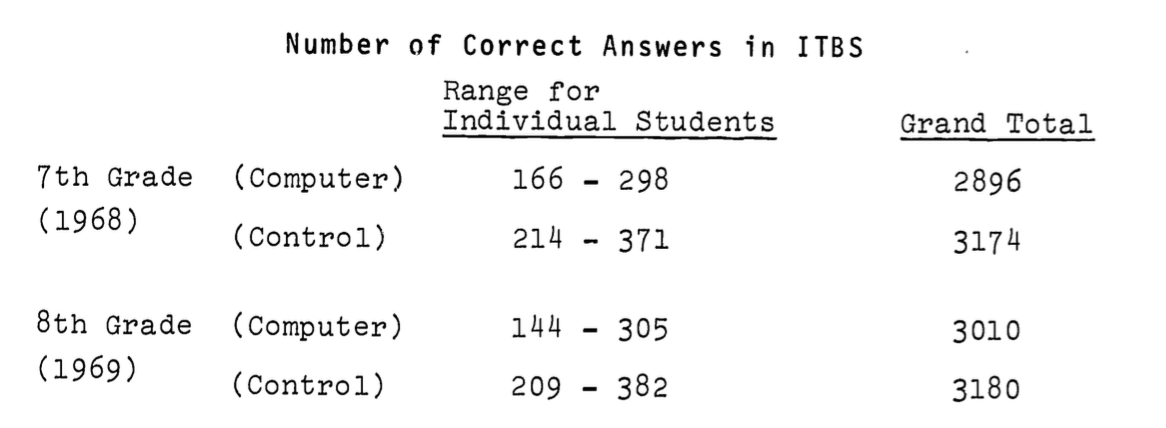
\includegraphics[width=0.8\textwidth]{images/logo-itbs.png}
			\caption{Tabla que muestra los resultados obtenidos en el ITBS por los alumnos que aprendierona programar (denominado \emph{computer}) y el grupo de control. Obtenido de \cite[p.251]{feurzeig1969programming}.}
				\label{tab:logo-itbs}
	\end{centering}
\end{table}


\subsection{Uso del lenguaje Logo}
\label{sec:logo-lenguaje}

A continuación se realizará una revisión de las principales características del lenguaje Logo para tener una visión general de su funcionamiento y sintaxis. Este análisis se basa en el trabajo de \cite[p.274-305]{feurzeig1969programming}. Si el lector quiere ampliar información sobre el lenguaje Logo, puede consultar \cite{friendly2014advanced} o \cite{logo-resources}.


\subsubsection*{\emph{words}, \emph{sentences}, operaciones y comandos}

Hay dos tipos de datos principales: \emph{words} y \emph{sentences}. \emph{words} está formado por 0 o más caracteres, sin espacios. Algunos ejemplos son: "SUN", "CAT", "5",  "97&!", "" (cadena vacía). El tipo de datos \emph{sentences} se forma por un conjunto de \emph{words} separado por espacios, como por ejemplo "HELLO WORLD" o "3 + 2 = 5". Un numero es una \emph{word} pero conpuesto únicamente por dígitos.

En el lenguaje Logo existen operadores para tratar con los tipos \emph{words} y \emph{sentences}. También se pueden encontrar una serie de operaciones predefinidas en el lenguaje que ofrecen funcionalidad extra, como controlar la entrada/salida de un programa, saber la fecha o manejo de \emph{words} y \emph{sentences}. En la tabla \ref{tab:logo-operaciones} vemos un resumen de las operaciones elementales del lenguaje Logo, el número de argumentos que requiere y un ejemplo de entrada con su salida correspondiente.


\begin{table}[!ht]
	\begin{centering}
		\begin{tabular}{c|c|c|c}
\emph{Operador} & N. argumentos & Entrada & Salida\\
\hline
\texttt{FIRST}	& 1 & "CAT" & "C"\\
- & - & "CAT AND DOG" & "CAT"\\
\texttt{LAST} & 1 & "CAT" & "T"\\
- & - & "CAT AND DOG" & "DOG"\\
\texttt{BUTFIRST} &1& "CAT" & "AT"\\
- & - & "CAT AND DOG" & "AND DOG"\\
\texttt{BUTLAST} & 1 & "CAT" & "CA"\\
- & - & "CAT AND DOG" & "CAT AND"\\
\texttt{COUNT} & 1 & "CAT" & "3"\\
- & - & "CAT DOG" & "2"\\
\texttt{WORD}& 2 & "CAT" "DOG" & "CATDOG"\\
\texttt{SENTENCE}& 2 & "CAT" "DOG" & "CAT DOG"\\
- & - & "CAT " "DOG" & "CAT DOG"\\
\texttt{PRINT} & 1 & "CAT" & CAT\\
\texttt{TIME} & 0 & - & "5:42 PM"\\
\texttt{DATE} & 0 & - & "1/31/2016"\\
\texttt{SUM} & 2 & "-5" "5" & "0"\\
\texttt{DIFFERENCE} & 2 & "5" "5"& "0"\\
\texttt{MAXIMUN} & 2 & "-5" "5" & "5"\\
\texttt{MINIMUN} & 2 & "3" "5"& "3"\\
\end{tabular}
	\caption{Resumen de las operaciones elementales que ofrece el lenguaje Logo.}
		\label{tab:logo-operaciones}
	\end{centering}
\end{table}

Si se intentara ejecutar la operación \texttt{WORD} "CAT " "DOG", se produciría un error al ser uno de sus parámetros un tipo \emph{sentence} y no \emph{word} (el primer argumento contiene un espacio). De igual manera, las operaciones \texttt{SUM}, \texttt{DIFFERENCE}, \texttt{MAXIMUN} y \texttt{MINIMUN} deben recibir argumentos numéricos o se produciría un error.

También es posible encadenar varios operadores. De esta manera, la cadena de instrucciones \texttt{FIRST OF BUTFIRST OF "CAT"} devolverá el \emph{word} "A".


\subsubsection*{Variables, comentarios y definiendo nuevas operaciones}
\label{sec:logo-variables}

Para definir variables basta con usar el operador \texttt{MAKE} seguido de \emph{"}(comilla doble), el nombre de la variable y el valor que se quiere asignar. Para hacer uso de la variable, utilizamos el símbolo \emph{:}(dos puntos) seguido del nombre de la variable. Para hacer comentarios se utiliza el símbolo \emph{;}(punto y coma). Podemos ver un ejemplo en el código \ref{code:logo-nueva-variable}.

\begin{lstlisting}[language={Logo}, label={code:logo-nueva-variable}, caption={Ejemplo de definición de nuevas variables en el lenguaje Logo.}]
MAKE "ADULTO 18

PRINT :ADULTO  ; salida -> 18
\end{lstlisting}

También es posible crear nuevas operaciones. Se utilizan las palabras reservadas \texttt{TO} y \texttt{END} para marcar el inicio y final de la definición, respectivamente. A continuación es necesario declarar el nombre con el que se definirá la operación que se está creando (el cual no puede coincidir con ninguna palabra reservada en el lenguaje, como es común en la mayoría de lenguajes de programación). Es opcional la declaración de parámetros que se pasaran a la operación. Por último, y antes de la palabra \texttt{END}, se incluirán las instrucciones que realizará la operación.

En el código \ref{code:logo-nuevas-operaciones} se puede ver un ejemplo de definición de nuevas operación.

\begin{lstlisting}[language={Logo}, label={code:logo-nuevas-operaciones}, caption={Definición de nuevas operaciones en el lenguaje Logo.}]
TO SALUDAR
	MAKE "SALUDO "HELLO WORLD"
	OUTPUT SALUDO
END

PRINT SALUDAR  ;  salida -> HELLO WORLD

TO PENULTIMO :algo
	OUTPUT FIRST OF  LAST :algo
END

PRINT PENULTIMO OF "CAT BIRD DOG" ;  salida  ->  BIRD

PRINT PENULTIMO OF "CAT" ;  salida  ->  A
\end{lstlisting}


\subsubsection*{Operadores aritméticos}

A parte de los operadores \texttt{SUM} y \texttt{DIFFERENCE} antes mencionados, Logo también otorga la posibilidad de utilizar los operadores aritméticos clásicos. La única condición es que la salida generada debe ser tratada (\texttt{PRINT}) o almacenada (en variables, como veremos en la sección siguiente) de alguna manera. Los operadores más importantes son \texttt{+}, \texttt{-}, \texttt{*}, \texttt{/} y \texttt{sqrt}.

\begin{lstlisting}[language={Logo}, label={code:logo-operadores-aritmeticos}, caption=Ejemplo de uso de operadores aritméticos en el lenguaje Logo.]
PRINT 2*3  ;  salida  -> 6

MAKE "RUEDAS  4

PRINT :RUEDAS ;  salida  -> 4
\end{lstlisting}


\subsubsection*{Operadores \texttt{IF} y \texttt{REPEAT}}

Se pueden crear operaciones condicionales utilizando la palabra clave \texttt{IF} seguida de una sentencia y una lista de órdenes a ejecutar si se evalúa dicha sentencia a verdadero. La lista de órdenes se declara entre corchetes (\texttt{[]}) y para la sentencia se pueden utilizar los operadores infijos \texttt{=}, \texttt{>} y \texttt{<}. En el código \ref{code:logo-if} podemos ver un ejemplo de uso.

\begin{lstlisting}[language=Logo,label={code:logo-if}, caption=Condiciones en el lenguaje logo con el operador \texttt{IF}.]
MAKE "PETALOS 4

IF :PETALOS > 3 [ PRINT "TREBOL DE LA BUENA SUERTE" ]
\end{lstlisting}

Para repetir una serie de instrucciones, Logo ofrece el comando \texttt{REPEAT}, que va seguido de un valor numérico y la lista de instrucciones. El valor numérico (que puede ser parametrizado) es el número de veces que se repetirá en bucle las instrucciones. En el código \ref{code:logo-repeat} vemos un ejemplo de este comando.


\begin{lstlisting}[language=Logo,label={code:logo-repeat}, caption=Condiciones en el lenguaje logo con el operador \texttt{IF}.]
REPEAT 10 [ PRINT "HOLA MUNDO" ]
\end{lstlisting}


\subsection{Turtle de Logo}
\label{sec:turtle}

El proyecto \emph{Turtle} es el proyecto más popular del lenguaje Logo. Nació como una criatura robótica, arreglada para que pareciera una tortuga, que se movía por el suelo con un rotulador atado que pintaba el suelo. Más tarde evolucionó a una imagen de una tortuga que se movía por la pantalla pintando según se desplazaba. Turtle se utiliza ampliamente desde hace décadas para enseñar a programar a niños de Primaria y Secundaria conceptos de programación, pero también de matemáticas y geometría\cite{abelson1980disessa,brown1995101}.

A pesar de su larga vida, el proyecto Turtle ha sabido mantenerse vivo y se ha modernizado en proyectos más recientes como Turtle Academy \cite{turtle-academy} o Curly Logo \cite{curly-logo}.


\subsubsection{Programando el movimiento de Turtle en el lenguaje Logo}
\label{sec:logo-turtle-lenguaje}

A parte de toda la funcionalidad que ofrece Logo como lenguaje, Turtle aporta una librería para poder controlar a nuestra criatura que pintará la pantalla. Ésta suele ser tradicionalmente representada con una tortuga o una flecha. Principalmente, se podrá controlar el movimiento de nuestra tortuga y el giro de ésta. También se le podrá ordenar que deje de pintar para permitir movimiento por la pantalla sin rastro. La mayoría de estos comandos pueden abreviarse para simplificar la escritura.

El resumen sobre la funcionalidad de Turtle que se muestra en las secciones siguientes es un compendio formado a partir de \cite{logo-turtle-lenguaje}, \cite{turtle-academy} y \cite{abelson1980disessa}.


\subsubsection*{Moviendo a Turtle}

La tortuga siempre se moverá según el eje de coordenadas. El punto (0, 0) se encontrará normalmente en medio de la pantalla y es la posición inicial de la tortuga. El eje de coordenadas \texttt{y} crece positivamente en dirección Norte (hacia arriba).

Los comandos \texttt{forward} y \texttt{barckward} mueven la tortuga hacia delante y atrás, respectivamente, según la posición en la que esté mirando. Los comandos \texttt{setx}, \texttt{sety} y \texttt{setxy} se utilizan para establecer la tortuga en el eje de coordenadas \texttt{x}, \texttt{y} o en ambos, respectivamente.

La orden \texttt{home} devuelve a la tortuga a la posición (0, 0) de la pantalla. Adicionalmente, se puede ocultar o mostrar (si ya está oculta) la tortuga con las órdenes \texttt{showturtle} y \texttt{hideturtle}.

Otra función muy importante de Turtle, es la opción de girarla. Podemos decidir el giro con las instrucciones \texttt{right} y \texttt{left} y el ángulo de giro (el valor tiene que ser un número positivo). Un ángulo de giro de 380º sería equivalente a girar la tortuga 20º.


\subsubsection*{Pintando con Turtle}

Hasta ahora, cualquier desplazamiento de Turtle por la pantalla dejaba una linea o rastro. Con la orden \texttt{penup}, la tortuga dejará de pintar hasta que se ejecute la orden \texttt{pendown}. También se puede ejecutar la instrucción \texttt{clearscreen} que limpiará la pantalla de cualquier rastro dejado por la tortuga.

La instrucción \texttt{label} acepta un argumento y mostrará por pantalla su contenido. El argumento debe ser de tipo \emph{word} o \emph{sentence}\footnote{Para más información sobre los tipos de datos \emph{words} y \emph{sentences}, como se formar y cual es su funcionamiento, se puede consultar la sección \ref{sec:logo-variables}.}.

\subsubsection*{Resumen de instrucciones de Turtle}


En la tabla \ref{tab:turtle-lenguaje} se muestra un resumen de las órdenes que puede recibir Turtle.

\begin{table}[!ht]
	\begin{centering}
		\begin{tabular}{c|c|c}
Orden & abreviatura & Argumentos\\
\hline
forward & fd & Longitud del movimiento\\
backward & bk & Longitud del movimiento\\
home & - & -\\
setx & - & Nueva coodenada X\\
sety & - & Nueva coodenada Y\\
setxy & - & Nueva coodenada X e Y\\
right & rt & Ángulo en el sentido de las agujas del reloj\\
left & lt & Ángulo en el sentido contrario a las agujas del reloj\\
penup & pu & -\\
pendown & pd & -\\
clearscreen & cs & -\\
label & - & Una \emph{word} o \emph{sentence}\\
showturtle & st & -\\
hideturtle & ht & -\\
\end{tabular}
	\caption{Resumen de órdenes en Turtle usando el lenguaje Logo.}
		\label{tab:turtle-lenguaje}
	\end{centering}
\end{table}









%%%%%%%%%%%%%%%%%%%%%%%%%%%%%%%%%%%%%%%%%%%%%%
%%%%%%%%%%%%%%%%%%%%%%%%%%%%%%%%%%%%%%%%%%%%%%%%%%%%%%%%%%%%%%%%%%%%%%%%%%%%%%%%%%%%%%%%%%%%
%%%%%%%%%%%%%%%%%%%%%%%%%%%%%%%%%%%%%%%%%%%%%%%%%%%%%%%%%%%%%%%%%%%%%%%%%%%%%%%%%%%%%%%%%%%%
%%%%%%%%%%%%%%%%%%%%%%%%%%%%%%%%%%%%%%%%%%%%%%

{\color{green}
(J.A.:) ¿Comentarás algo de robomind o codehs que también son descendientes directos de lego? lo bueno es que el primero te hace enfocar la idea de la tortuga hacia un robot más realista, la segunda que lleva el aprendizaje a entorno web y tecnologías javascript. Todo esto te abre temas para seguir escribiendo el trabajo. Recuerda que sabes más de lo que crees y has hecho más de lo que piensas.
}


% \section{Khan Academy}
% \label{sec:Khan Academy}

% Khan Academy\cite{khan-academy}, con casi 37 millones de usuarios, es uno de los mayores proyectos web para aprender casi de cualquier tema: Matemáticas, estadística, economía o humanidades.


% \section{Code.org}
% \label{sec:Code.org}

% Code.org\cite{code-org} es una plataforma on-line que se dedica exclusivamente a enseñar a programar y cuenta ya con más de 8 millones de usuarios. Cuenta con una gran comunidad de educadores y apoyos entre los que se puede contar al Presidente B. H. Obama. Lleva a cabo proyectos como \emph{Hour of Code} en el que promueve que los usuarios inviertan una hora diaria programando en diferentes juegos, muchos de ellos utilizando \Gls{Blockly}\cite{blockly}.


% \section{Squeak Etoys}
% \label{sec:squeak-etoys}


% \section{Blockly y Scratch}
% \label{sec:blockly-scratch}


%%%%%%%%%%%%%%%%%%%%%%%%%%%%%%%%%%%%%%%%%%%%%%%%
% 3: Análisis de objetivos y metodología
%%%%%%%%%%%%%%%%%%%%%%%%%%%%%%%%%%%%%%%%%%%%%%%%
\chapter{Análisis de objetivos y metodología}\label{objetivos-metodologia}

\section{Objetivos}
\label{sec:Objetivos}

Este Trabajo Fin de Grado consiste en desarrollar un módulo de simulación de un robot para integrarlo en la plataforma \Gls{descubre}. Para ello se tendrán que cubrir una serie de subobjetivos que nombraremos a continuación.
\begin{itemize}
\item Estudiar el uso y aplicación de diferentes librerías de físicas para generar el robot.
\item Comprensión de la plataforma Descubre así como su posterior modificación.
\item Creación de un simulador de un robot de dos ruedas y su integración en la plataforma Descubre.
\item Modificación del motor de \gls{ijava} y creación de la \acrshort{API} para poder controlar el robot.
\end{itemize}

\section{Metodología}
\label{sec:metodologia}

{\color{green}
Que metodología he seguido? Extreme programming


Hablar de herramientas utilizadas?
}

%%%%%%%%%%%%%%%%%%%%%%%%%%%%%%%%%%%%%%%%%%%%%%%%
% 4: Diseño y resolución del trabajo realizado
%%%%%%%%%%%%%%%%%%%%%%%%%%%%%%%%%%%%%%%%%%%%%%%%
\chapter{Diseño y resolución del trabajo realizado}\label{diseno}


{\color{green}
Decidir que poner, como, en que orden.
}



%%%%%%%%%%%%%%%%%%%%%%%%%%%%%%%%%%%%%%%%%%%%%%%%
% 5: Conclusiones y vías futuras
%%%%%%%%%%%%%%%%%%%%%%%%%%%%%%%%%%%%%%%%%%%%%%%%
\chapter{Conclusiones y vías futuras}\label{conslusiones}




{\color{blue}
explicar en que se diferencia robode con el resto y porque es mejor o que ventajas tiene
explicar como resuelvo los problemas que se encuentra un estudiante cuando programa (intro-3º parrafo)
}
